\documentclass[final,hyperref={pdfpagelabels=false}]{beamer}

\usepackage[T1]{fontenc}
\usefonttheme{professionalfonts}
\usepackage[sfmath,slantedGreeks]{kpfonts}
\usepackage[utf8]{inputenc}
\usepackage[orientation=portrait,size=a0,scale=1.4]{beamerposter}
\usepackage{graphicx,pifont,siunitx}

% \usetheme{Madrid}
\usecolortheme{beaver}
\setbeamertemplate{navigation symbols}{}

% Customise the caption: do not insert the caption name, nor the number, just
% insert a smaller caption text.
\setbeamertemplate{caption}{\scriptsize\insertcaption}

% % beaver è un tema grigio-rosso, ma non cambia il colore dei bullet di itemize e
% % di enumerate.  Il seguente comando serve a impostarli al colore darkred
% % definito nel tema beaver.
% \setbeamercolor{structure}{fg=darkred}

% \definecolor{darkblue}{rgb}{0,0,0.8}

%%%%%%%%%%%%%%%%%%%%%%%%%%%%%%%%%%%%%%%%%%%%%%%%%%%%%%%%%%%%%%%%%%%%%%%%%%%%%%%%
%%%%%%%%%%%%%%%%%%%%%%%%%%%%%%%%%%%%%%%%%%%%%%%%%%%%%%%%%%%%%%%%%%%%%%%%%%%%%%%%
%%%%%%%%%%%%%%%%%%%%%%%%%%%%%%%%%%%%%%%%%%%%%%%%%%%%%%%%%%%%%%%%%%%%%%%%%%%%%%%%

% Colors
\RequirePackage{tangocolors}
\selectcolormodel{cmyk}

\setbeamercolor{headline}{fg=tabutter,bg=black}
\setbeamercolor{footline}{fg=tabutter, bg=ta3gray}
\setbeamerfont{footline}{size=\large}
\setbeamercolor{separation line}{bg=ta2orange}
\setbeamercolor{title in headline}{fg=tabutter}
\setbeamercolor{author in headline}{fg=ta2orange}
\setbeamercolor{institute in headline}{fg=ta3orange}

\setbeamercolor{framesubtitle}{fg=ta3orange, bg=ta2gray}
\setbeamercolor{author in head/foot}{fg=ta2orange, bg=black}
\setbeamercolor{title in head/foot}{fg=ta2orange, bg=black}

\setbeamercolor*{normal text}{fg=tachameleon, bg=ta3gray}
\setbeamercolor*{block body}{bg=ta3aluminium,fg=black}
\setbeamercolor*{block title}{fg=taorange,bg=ta2gray}
\setbeamerfont{block title}{size=\large,series=\bf}
\setbeamercolor{upper separation line head}{fg=ta2orange}

\setbeamercolor*{example body}{fg=ta3aluminium,bg=black}
\setbeamercolor*{example text}{fg=ta3aluminium,bg=black}
\setbeamercolor*{example title}{bg=taorange,fg=ta2gray}

\setbeamercolor{alerted text}{fg=ta3gray}

%\setbeamercolor{example text}{fg=taorange}
\setbeamercolor{structure}{fg=ta3gray}

% adapt height of imtemize rectangles
\setbeamertemplate{itemize items}[ball]
% \setbeamertemplate{itemize item}{\raisebox{0.12ex}{$\blacktriangleright$}\hskip.1em}
% \setbeamertemplate{itemize subitem}{\raisebox{0.12ex}{$\triangleright$}\hskip.1em}
% or define your own template using \defbeamertemplate{itemize item}, see beameruserguide.pdf

% equal font sizes for all levels
\setbeamerfont{itemize/enumerate body}{size=\normalsize}
\setbeamerfont{itemize/enumerate subbody}{size=\normalsize}
\setbeamerfont{itemize/enumerate subsubbody}{size=\normalsize}

% Templates
% \setbeamertemplate{block begin}{
%   \vskip.75ex
%   \begin{beamercolorbox}[ht=3.5ex,dp=0.5ex,center,leftskip=-1em,colsep*=.75ex]{block title}%
%     \usebeamerfont*{block title}%
%     {\phantom{Gg}\insertblocktitle}% phantom because of baseline problem
%   \end{beamercolorbox}%
%   {\ifbeamercolorempty[bg]{block body}{}{\nointerlineskip\vskip-0.5pt}}%
%   \usebeamerfont{block body}%
%   \begin{beamercolorbox}[leftskip=1em,colsep*=.75ex,sep=0.5ex,vmode]{block body}%
%     \ifbeamercolorempty[bg]{block body}{\vskip-.25ex}{\vskip-.75ex}\vbox{}%
%   }
%   \setbeamertemplate{block end}{
%   \end{beamercolorbox}
% }

\setbeamertemplate{headline}{
  \leavevmode
  \begin{beamercolorbox}[wd=\paperwidth]{headline}
    \begin{columns}[T]
      \begin{column}{0.02\paperwidth}
      \end{column}
      \begin{column}{.12\paperwidth}
        \begin{center}
          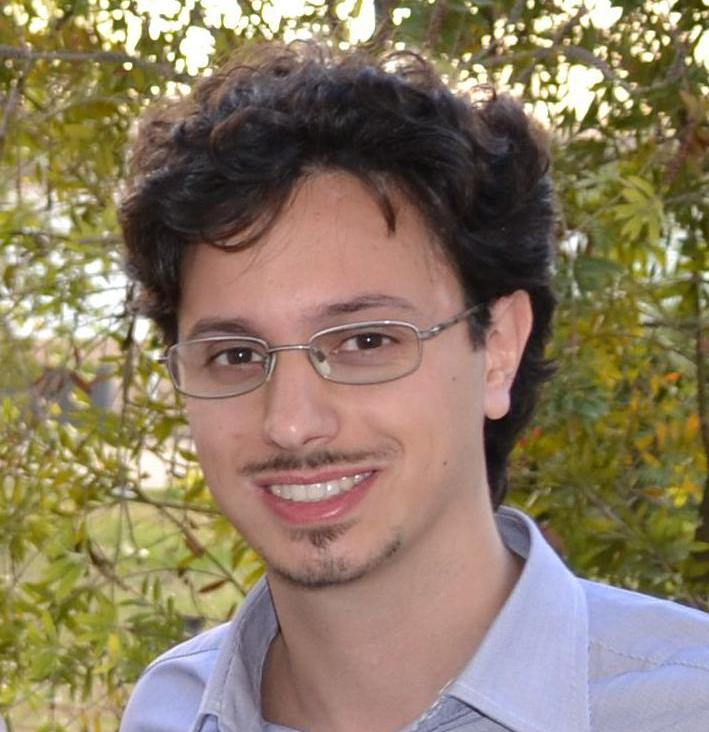
\includegraphics[width=\columnwidth]{figures/giordano.jpg}
        \end{center}
      \end{column}
      \begin{column}{.7\paperwidth}
        \vskip4ex
        \raggedleft
        \usebeamercolor{title in headline}{\color{fg}\textbf{\Huge{\inserttitle}}\\[1ex]}
        \usebeamercolor{author in headline}{\color{fg}\Large{\insertauthor}\\[1ex]}
        \usebeamercolor{institute in headline}{\color{fg}\large{\insertinstitute}\\[1ex]}
      \end{column}
      \begin{column}{.16\paperwidth}
        \vskip4ex
        \begin{center}
          
\includegraphics[width=.4\columnwidth]{figures/logo-unisalento.pdf} \qquad
          
\includegraphics[width=.4\columnwidth]{figures/infn.jpg} \\[3ex]
          
\includegraphics[width=.88\columnwidth]{figures/dipartimento.png}
        \end{center}
        \vskip2ex
      \end{column}
      \begin{column}{.02\paperwidth}
      \end{column}
    \end{columns}
    \vskip2ex
  \end{beamercolorbox}

  \begin{beamercolorbox}[wd=\paperwidth]{lower separation line head}
    \rule{0pt}{3pt}
  \end{beamercolorbox}
}

\setbeamertemplate{footline}{
  \begin{beamercolorbox}[wd=\paperwidth]{upper separation line foot}
    \rule{0pt}{3pt}
  \end{beamercolorbox}

%  \leavevmode%
  \begin{beamercolorbox}[ht=4ex,leftskip=1em,rightskip=1em]{author in head/foot}%
    \textsc{Mosè Giordano} (University of Salento and INFN Lecce)
    \hfill
    La Palma, Canary Islands, \insertdate
    \vskip0.9ex
  \end{beamercolorbox}
  \vskip0pt%
  \begin{beamercolorbox}[wd=\paperwidth]{lower separation line foot}
    \rule{0pt}{3pt}
  \end{beamercolorbox}
}

%%%%%%%%%%%%%%%%%%%%%%%%%%%%%%%%%%%%%%%%%%%%%%%%%%%%%%%%%%%%%%%%%%%%%%%%%%%%%%%%
%%%%%%%%%%%%%%%%%%%%%%%%%%%%%%%%%%%%%%%%%%%%%%%%%%%%%%%%%%%%%%%%%%%%%%%%%%%%%%%%
%%%%%%%%%%%%%%%%%%%%%%%%%%%%%%%%%%%%%%%%%%%%%%%%%%%%%%%%%%%%%%%%%%%%%%%%%%%%%%%%


\newcommand{\arxiv}[1]{{\usebeamercolor[fg]{bibliography entry note}
    \href{http://arxiv.org/abs/#1}{arXiv: \texttt{#1}}}}
\newcommand{\doi}[1]{{\usebeamercolor[fg]{bibliography entry note}
    \href{http://dx.doi.org/#1}{\textsc{doi}: \texttt{#1}}}}

\DeclareMathOperator{\e}{\mathrm{e}}
\DeclareMathOperator{\uimm}{\mathrm{i}} % unità immaginaria
\renewcommand{\phi}{\varphi}
\renewcommand{\epsilon}{\varepsilon}
% complesso coniugato: \conjg{z}
\newcommand{\conjg}[1]{\overline{#1}}
\newcommand{\tah}[1]{\tilde{#1}}
% Nelle presentazioni il neretto non si distingue bene, ridefinisco \bm come \vec
\newcommand*{\dd}{\mathop{}\!\textup{d}} % Operatore differenziale \dd
% Derivata totale: \toder[ordine]{funzione}{variabile}
\newcommand*{\toder}[3][]{\frac{{\dd^{#1}}#2}{\dd {#3}^{#1}}}
\newcommand*{\ltoder}[3][]{{\dd^{#1}}#2/\dd {#3}^{#1}}

% Simboli che si possono utilizzare negli elenchi dell'ambiente itemize.  `\pro'
% (nel senso di "vantaggio") produce un tick, `\con' (nel senso di "contro")
% produce un cross.  Usa simboli del pacchetto `pifont'
\newcommand{\pro}{\color{alerted text.fg}{\ding{51}}}
\newcommand{\con}{\color{alerted text.fg}{\ding{55}}}

\title{Estimating orbital period of exoplanets \\
  in microlensing events}
\author{Achille A. Nucita, \emph{Mosè Giordano}, Francesco De Paolis, Gabriele
  Ingrosso}
\institute[University of Salento and INFN Lecce]{Department of Mathematics and
  Physics ``\emph{E. De Giorgi}'', University of Salento, Lecce, Italy \\
  INFN, Section of Lecce, Italy}
\date{24--25 September 2014}

\begin{document}
\begin{frame}
  \begin{columns}
    %%% Left column
    \begin{column}{0.48\columnwidth}
      \begin{minipage}[T]{\columnwidth}
        \begin{block}{Gravitational lensing}
          A \alert{gravitational lens} is a distribution of matter whose
          gravitational pull distorts space-time, bends light rays and
          \alert{amplifies} the luminosity of a source star coming to an
          observer
          \begin{figure}
            \centering
            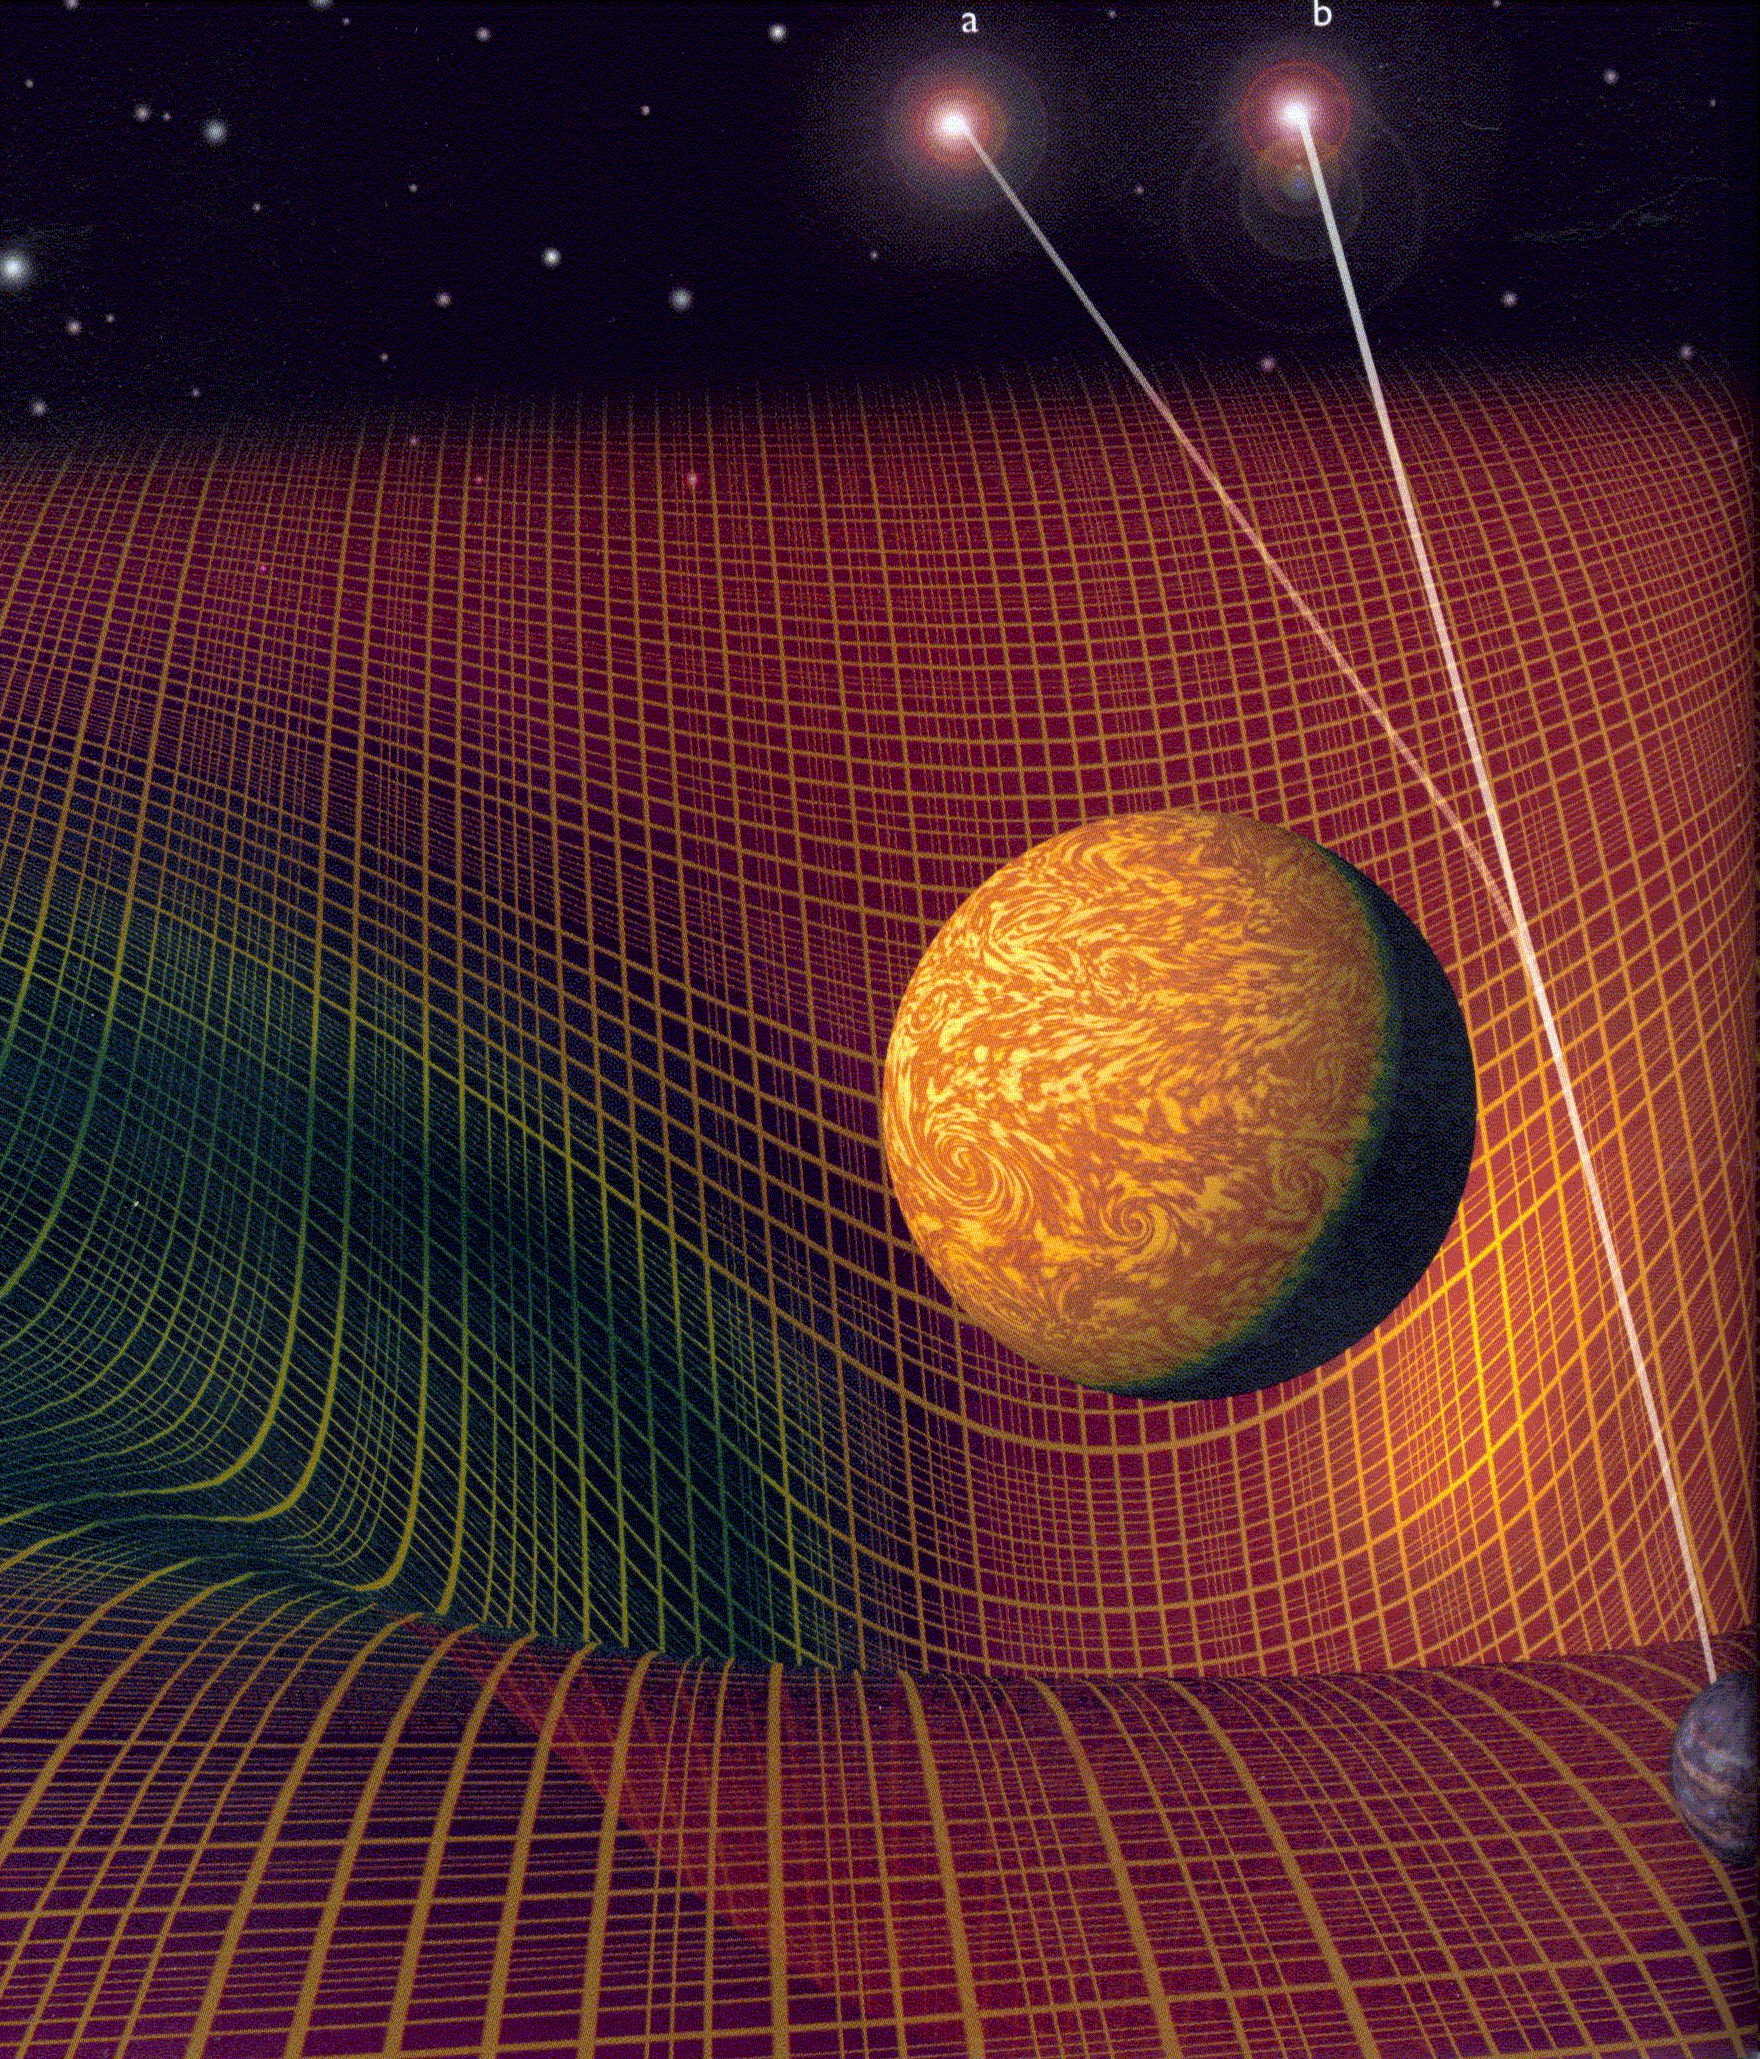
\includegraphics[width=0.5\columnwidth]{figures/Spacetime.jpeg}
            \caption{Credits: Hyper-Mathematics - Uzayzaman / Spacetime}
            \vspace{-0.5em}
          \end{figure}
        \end{block}
        
        \begin{block}{Binary Lens with Orbital Motion}
          Usually, in microlensing events static binary systems are taken into
          account, but binary systems do rotate

          The parameters to be determined using a fit in microlensing events by
          binary lens with orbital motion are
          \begin{itemize}
          \item Paczyński curve parameters: \(t_{0} \quad u_{0} \quad
            t_{\textup{E}} \quad \theta\)
          \item finite source effects: \(\rho_{\star}\)
          \item binary lens: \(b \quad q\)
          \item binary lens with orbital motion: \(a \quad e \quad i \quad
            \phi\)
          \end{itemize}
          In addition, with small mass ratios \(q\) there is the
          \alert{close-wide degeneracy} \(b \longleftrightarrow b^{-1}\)

          What if we knew the orbital period of the lenses
          \begin{equation*}
            P = 2\pi\sqrt{\frac{a^{3}}{GM}} =
            2\pi\sqrt{\frac{a^{3}}{Gm_{1}(1 + q)}}
          \end{equation*}
          \alert{independently}?
        \end{block}

        \begin{block}{Fit to Real Data}
          \begin{figure}
            \centering
            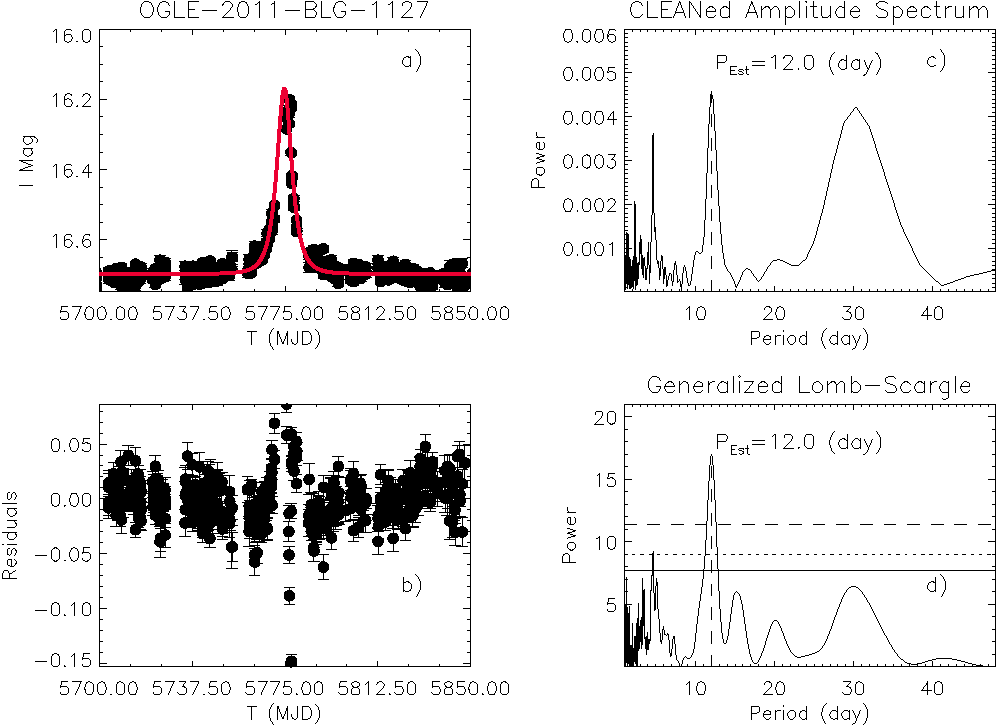
\includegraphics[width=0.7\textwidth]{figures/ogle322all}
            \caption{Event OGLE-2011-BLG-1127/MOA-2011-BLG-322}
            \vspace{-0.5em}
          \end{figure}
        \end{block}

        \begin{block}{Discussion}
          \begin{itemize}
          \item[\pro] Orbital period of the lenses should be \alert{shorter}
            than the Einstein time or we must have \alert{long observational
              window}
          \item[\pro] We fit the observed amplification curve to a \alert{simple
              Paczyński curve}, with four easily-guessable free parameters, and
            then perform a periodogram on the reside curve: the deduced period
            is the \alert{period of the binary system}
          \item[\pro] We need to \alert{remove a very small region} around the
            maximum amplification peak from the residue curve to perform the
            periodogram
          \item[\con] Periodic feature with the same period far from the peak
            \(\implies\) \alert{source periodicity} (binary system, intrinsic
            variable, etc\dots)
          \end{itemize}
        \end{block}
      \end{minipage}
    \end{column}

    %%% Right column
    \begin{column}{0.48\textwidth}
      \begin{minipage}[T]{\columnwidth}
        \begin{block}{Detecting Exoplanets with Microlensing}
          \alert{Microlensing} is a powerful tool to detect exoplanets: a binary
          system (lensing star with a companion planet) induces non-negligible
          deviations to the usual symmetric \alert{Paczyński light curve}
          \begin{figure}
            \centering
            % http://www.nature.com/nature/journal/v439/n7075/fig_tab/439400a_F2.html
            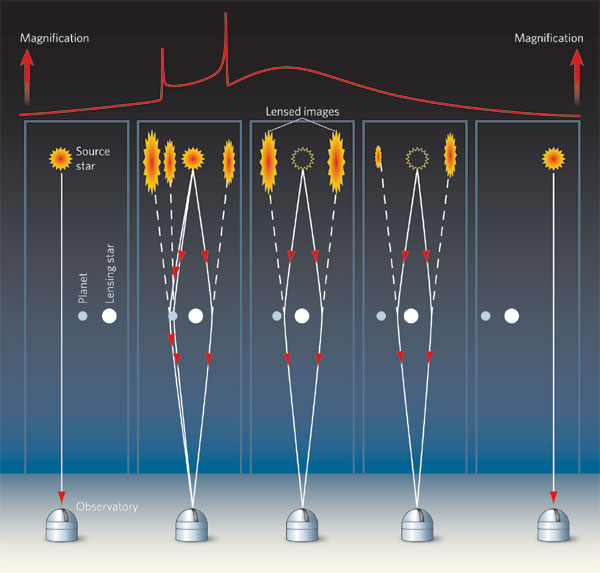
\includegraphics[width=.615\columnwidth]{figures/microlensing.jpg}
            \caption{Credits: Didier Queloz, \emph{Nature} \textbf{439},
              400--401.  \doi{10.1038/439400a}}
            \vspace{-0.5em}
          \end{figure}
        \end{block}

        \begin{block}{Simulation: Amplification Curve and Periodogram}
          \begin{figure}
            \centering
            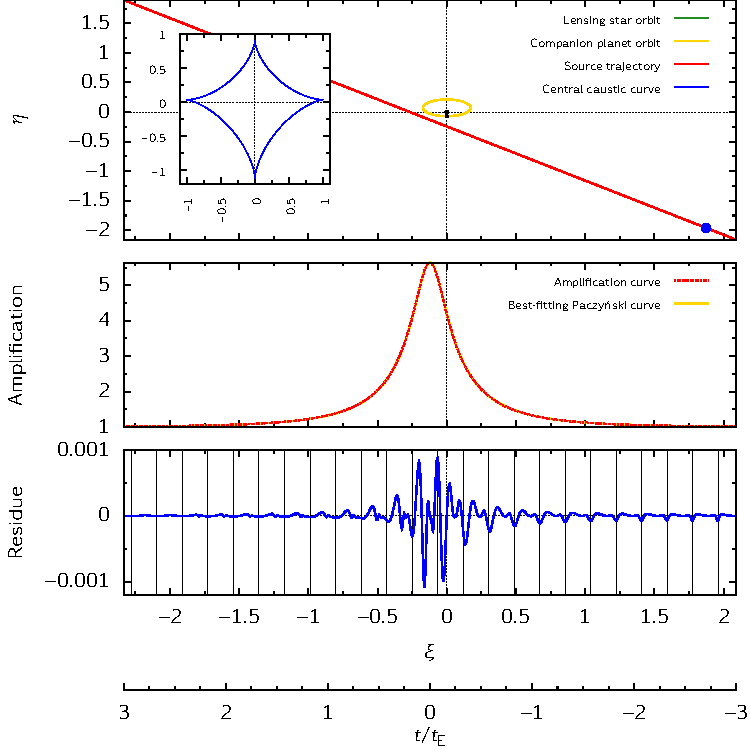
\includegraphics[width=0.775\columnwidth]{figures/figure2}\\[1.8ex]
            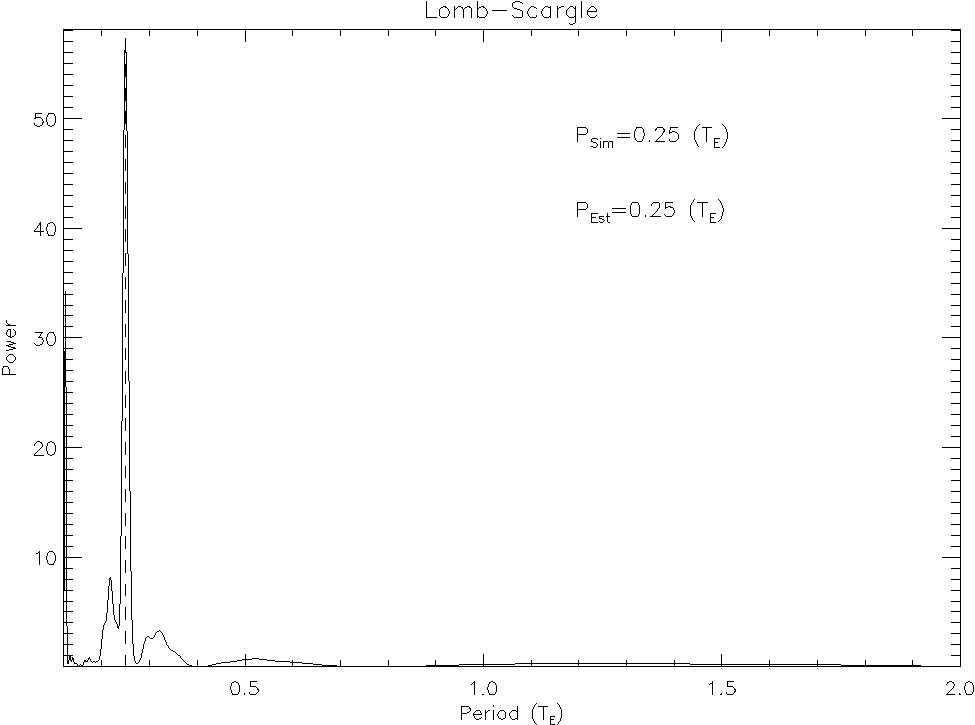
\includegraphics[width=0.775\columnwidth]{figures/lombscargle2}
            \caption{Parameters used: \(q = 10^{-3}\), \(a = 0.2\), \(e = 0.5\),
              \(i = \SI{45}{\degree}\), \(\phi = \SI{0}{\degree}\), \(P =
              t_{\textup{E}}/4\)}
            \vspace{-0.5em}
          \end{figure}
        \end{block}

        \begin{block}{Reference}
          \begin{itemize}
          \item[{
\includegraphics[scale=2]{figures/beamericonarticle-crop.pdf}}]
            A. A. Nucita, M. Giordano, F. De Paolis, and
            G. Ingrosso. ``\emph{Signatures of rotating binaries in microlensing
              experiments}''. In: \emph{Monthly Notices of the Royal
              Astronomical Society} 438 (Mar. 2014), pp. 2466–2473.
            \doi{10.1093/mnras/stt2363}. \arxiv{1401.6288}.
          \end{itemize}
        \end{block}
      \end{minipage}
    \end{column}
  \end{columns}
\end{frame}
\end{document}

%%% Local Variables:
%%% mode: latex
%%% TeX-master: t
%%% ispell-local-dictionary: "british"
%%% End:
